\section{Нелинейно-оптические процессы второго порядка в оптических волокнах}\label{sec:nlin2}

\subsection{Укороченные уравнения ГВГ}\label{subsec:shorted_shg}

Как указано в \cref{subsec:propagation}, нелинейный отклик среды описывается разложением поляризации $\mathbf{P}$ по степеням поля $\mathbf{E}$ (см.~\cref{eq:polarization}). Восприимчивость второго порядка $\chi^{(2)}$ даёт вклад в поляризацию на частоте $2\omega$:

\begin{equation}\label{eq:p_nl_chi2}
	\mathbf{P}^{(2)}(2\omega) = \varepsilon_0 \chi^{(2)} : \mathbf{E}(\omega)\mathbf{E}(\omega).
\end{equation}


\begin{equation}\label{eq:plane_wave}
	\mathbf{E}_\omega = \tfrac12 \mathbf{A}_1(z) e^{i(k_1 z - \omega t)} + \text{к.с.}, \qquad
	\mathbf{E}_{2\omega} = \tfrac12 \mathbf{A}_2(z) e^{i(k_2 z - 2\omega t)} + \text{к.с.}
\end{equation}

Для вывода укороченных уравнений ГВГ~\cite{dmitriev2004prikladnaya} представим поля основной волны и второй гармоники в виде плоских волн~\cref{eq:plane_wave} и подставим их в волновое уравнение~\cref{eq:wave} с нелинейной поляризацией~\cref{eq:p_nl_chi2}.  При выводе пользуемся приближением медленно меняющихся амплитуд, то есть пренебрегаем вторыми производными полей по координатам. Это справедливо при условии $|\partial^2 A_{1,2}/\partial z^2| \ll k_{1,2}|\partial A_{1,2}/\partial z|$. В случае ОВ необходимо заменить показатели преломления на эффективные показатели преломления соответствующих мод, а также учесть интегралы перекрытия поперечных распределений полей (см.~\cref{subsec:modes}). Итоговая система принимает вид:

\begin{subequations}\label{eq:shg_coupled}
	\begin{align}
		\frac{dA_1}{dz} &= \im \frac{2\pi\omega}{c n_\omega^{\text{eff}}} \chi^{(2)} \Gamma_1 A_1^* A_2 e^{-i\Delta k z}, \\
		\frac{dA_2}{dz} &= \im \frac{4\pi\omega}{c n_{2\omega}^{\text{eff}}} \chi^{(2)} \Gamma_2 A_1^2 e^{i\Delta k z},
	\end{align}
\end{subequations}

где $\Delta k = k_2 - 2k_1$ — волновая расстройка, а $\Gamma_{1,2}$~---интегралы перекрытия поперечных распределений полей взаимодействующих мод. В случае ГВГ в ОВ, как будет сказано далее, эти коэффициенты определяются перекрытием мод фундаментального излучения, второй гармоники и пространственного распределения наведённого статического поля $E_0$, создающего эффективную восприимчивость $\chi^{(2)} \sim \chi^{(3)} E_0$.

\subsection{Первые наблюдения и ключевые эксперименты}\label{subsec:first_observations}

Долгое время считалось, что в оптических волокнах из плавленого кварца нелинейно-оптические процессы второго порядка невозможны. Кварцевое стекло является центросимметричным на макроскопическом уровне в силу своей аморфной структуры (хотя кристаллический кварц обладает тригональной сингонией). Наблюдавшуюся слабую генерацию второй гармоники в таких средах объясняли поверхностными эффектами на границе сердцевина--оболочка и квадрупольной нелинейной поляризуемостью. Помимо электродипольного механизма, существуют также магнитный дипольный, электрический квадрупольный и поверхностный вклады, однако суммарная эффективность н-о преобразования, основанная на этих эффектах, согласно расчётам не превышает $10^{-3}\%$ \cite{terhune1987second}. Таким образом, за эффективное протекание процесса отвечают какие-то другие физические механизмы.


Существенный прогресс в понимании природы н-о эффектов второго порядка в центросимметричных средах наступил в 1986 году, когда Остерберг и Маргулис сообщили об увеличении эффективности генерации второй гармоники при длительном распространении излучения накачки по стандартному одномодовому ОВ, легированному германием. \cite{osterberg1986dye}. В течение 10~часов мощность второй гармоники возрастала практически экспоненциально, а затем выходила на насыщение. Эффективность преобразования достигала $3 \%$. В качестве накачки использовалось излучение твердотельного $\text{YAG:Nd}^{3+}$ лазера с длиной волны $\lambda = 1064~\text{нм}$, модуляцией добротности и пиковой мощностью до 20~кВт. Процесс роста мощности излучения второй гармоники ($\lambda = 532~\text{нм}$) получил название самоприготовления световода.

Работа Остерберга и Маргулиса дала старт интенсивным исследованиям в данной области. В 1987 году, основываясь на экспериментах с волокнами, легированными различными примесями, авторы работы \cite{farries1987second} постулировали механизм ГВГ как самоорганизующегося процесса формирования пространственной решётки дипольных центров окраски с периодом, соответствующим эффективной генерации второй гармоники. Также впервые была измерена кривая фазового синхронизма процесса и таким образом обнаружена спектральная зависимость эффективности генерации в <<самоприготовленном>> волокне. К настоящему времени общепризнано, что эффективная генерация второй гармоники в волокне обусловлена формированием пространственной решётки квадратичной нелинейности. Однако физический механизм возникновения такой решётки остаётся предметом активных дискуссий.

Важным этапом в развитии представлений о физических механизмах н-о эффектов в волокнах являлась работа Столена и Тома \cite{stolen1987self}, согласно которой знакопеременная решётка нелинейной восприимчивости второго порядка возникала за счёт ориентации дефектов на нулевой частоте (в постоянном электрическом поле). Постоянная же поляризация, а вследствие неё и постоянное поле, появляется в результате параметрического процесса третьего порядка, в котором излучение накачки и второй гармоники (возникающей из оптического шума либо привнесённой извне). В этом случае нелинейность второго порядка будет периодичной по пространству с периодом, соответствующим периоду синхронизма для генерации второй гармоники, а величина нелинейности (и эффективность преобразования) будет пропорциональна квадрату поля волны накачки и полю волны второй гармоники:

Статическая поляризация, возникающая при смешении волн на кубической нелинейности, имеет вид:

\begin{equation}\label{eq:stolen_pdc}
	P_{dc} = \frac{3}{8} \varepsilon_0 \chi^{(3)}(0 = \omega + \omega - 2\omega) |E_\omega|^2 E_{2\omega}^* \cos(\Delta k z),
\end{equation}

где $\Delta k = k_{2\omega} - 2k_\omega$~--- фазовая расстройка. Соответствующее электростатическое поле $E_{dc} = P_{dc}/(\varepsilon_0 \chi^{(1)})$ оказывается периодическим в пространстве с периодом $\Lambda = 2\pi/\Delta k$, что обеспечивает фазовый квазисинхронизм для ГВГ. Величина коэффициента квадратичной нелинейности при этом пропорциональна квадрату поля волны накачки и полю волны второй гармоники:

\begin{equation}\label{eq:stolen_chi2}
	\chi^{(2)} \propto |E_\omega|^2 E_{2\omega}^* \cos(\Delta k z + \varphi_p).
\end{equation}

Основываясь на зависимости нелинейной восприимчивости второго порядка от поля второй гармоники \cref{eq:stolen_chi2}, авторы работы~\cite{stolen1987self} предложили и осуществили эксперимент по генерации второй гармоники, вводя в оптическое волокно затравочное излучение на удвоенной в н-о кристалле частоте. При этом время установления эффективного преобразования уменьшилось с 12~часов до~5 минут. Как оказалось впоследствии, модель Столена и Тома не может описывать процесс ГВГ, так как максимальная величина постоянного поля возникающая при н-о процессах на кубической нелинейности, по порядку величины составляет $1~$В/см и недостаточна для эффективного протекания процесса~\cite{bergot1988generation}. Тем не менее, ключевой шаг в направлении понимания физики процесса был сделан (дальнейшие модели лишь показывают способы многократного усиления поля постоянной поляризации), а успех экспериментального подтверждения теоретических предположений, сделанных авторами в начале работы, направил дальнейшие усилия многих исследователей в сторону ориентационных моделей. 

В 1988~году Уллет с соавторами показали, что записанная решётка может быть стёрта оптически с использованием излучения второй гармоники, причём затухание не было экспоненциальным \cite{ouellette1988light}. Авторы предложили зарядовую модель, согласно которой  разделение зарядов возникает в постоянном электрическом поле, образованном параметрическим смешением частот накачки и второй гармоники. В отличие от модели Столена и Тома, где предполагалась ориентация диполей, зарядовая модель Уллета объясняла нелинейность через макроскопическое разделение зарядов и возникающее электростатическое поле. Это поле, согласно соотношению $\chi^{(2)} \sim \chi^{(3)} E_{dc}$, и создавало эффективную квадратичную восприимчивость.

Таким образом, в течение первых двух лет после обнаружения эффективной ГВГ в ОВ, были проведены основные экспериментальные исследования и предложены два класса физических моделей: зарядовые и ориентационные. Обе модели корректно описывали некоторые экспериментальные факты, однако вопрос о том, какая модель реализуется на практике, оставался открытым.






%\section{Физические модели фотоиндуцированной генерации второй гармоники в оптических волокнах}\label{sec:chFiber3/fibershg}
%\nomenclature{SHG}{Генерация второй гармоники}
%
%\todo{\subsection{Обзор существующих моделей ГВГ в ОВ}}
%\todo{\subsection{Роль фазового синхронизма при ГВГ в ОВ}}
%\todo{то что дальше будет частью главы про экспперименты}
%
%Итак, модели, объясняющие фотоиндуцированную генерацию второй гармоники в центросимметричных средах можно разделить на два класса~--- ориентационные и зарядовые. Важной характеристикой ориентационных моделей (рис. \ref{fig:models}, а) является предположение о том, что в среде ещё до включения лазерного излучения на микроскопическом уровне существует асимметрия дипольного типа. Под действием света происходит упорядочивание хаотически расположенных диполей. В зарядовых моделях (рис. \ref{fig:models}, б)  предполагается, что под действием лазерного излучения происходит фотоионизация зарядов, макроскопическое их разделение и формирование постоянного электрического поля, индуцирующего нелинейность второго порядка.
%
%\begin{figure}[h]
%	\centering
%	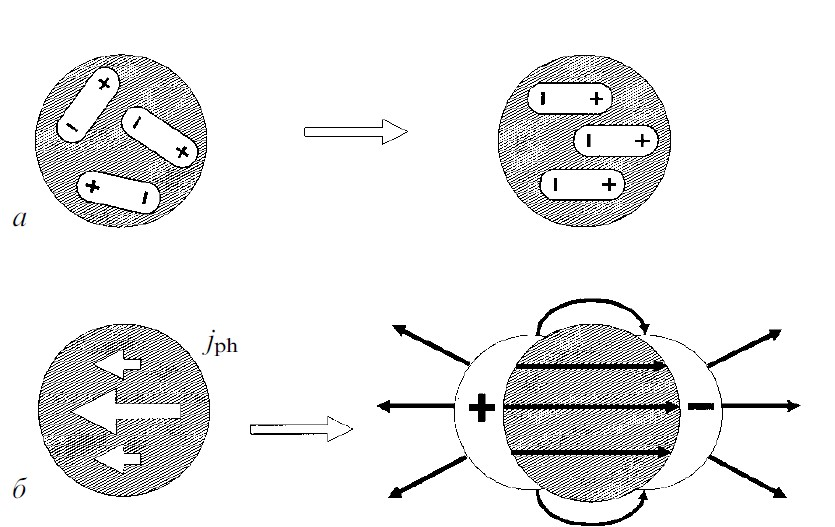
\includegraphics[width=0.6\linewidth]{Dissertation/images/review/models}
%	\caption{Возникновение фотоиндуцированного электрического поля в ориентационных (а) и зарядовых (б) моделях}
%	\label{fig:models}
%\end{figure}
%
%Важное отличие двух моделей заключается в характерных размерах области с ненулевым электрическим полем: в ориентационных моделях эта область сопоставима по размеру со световым пятном, в то время как в зарядовых моделях силовые линии электрического поля простираются значительно дальше освещённой области.
%
%Эксперимент, позволивший разделить два механизма, был проведён в 1992 году \cite{djanov1992photo}. Советский и российский учёный Евгений Дианов c коллегами предложили методику, основанную на существенной роли границы освещаемой области: при изменении граничного заряда в рамках зарядовой модели распределение электрического поля изменится значительно, а в рамках ориентационной~--- слабо. Из-за этого при смещении освещаемой области вдоль направления разделения зарядов представляется возможным создать протяжённую область заряда одного знака и малую~--- другого. При этом будут наблюдаться три максимума электрического поля (рис. \ref{fig:expsplit}, слева) и, как следствие, три максимума эффективности генерации гармоники. При движении в перпендикулярном направлении, равно как при работе в рамках ориентационной модели, зарядовые области будут одного размера и область эффективной генерации также будет однородной. Эксперимент подтвердил предположения авторов (рис. \ref{fig:expsplit}, справа)), и зарядовые модели стали доминирующими среди прочих предлагаемых физических механизмов генерации второй гармоники в оптическом волокне.
%
%\begin{figure}
%	\centering
%	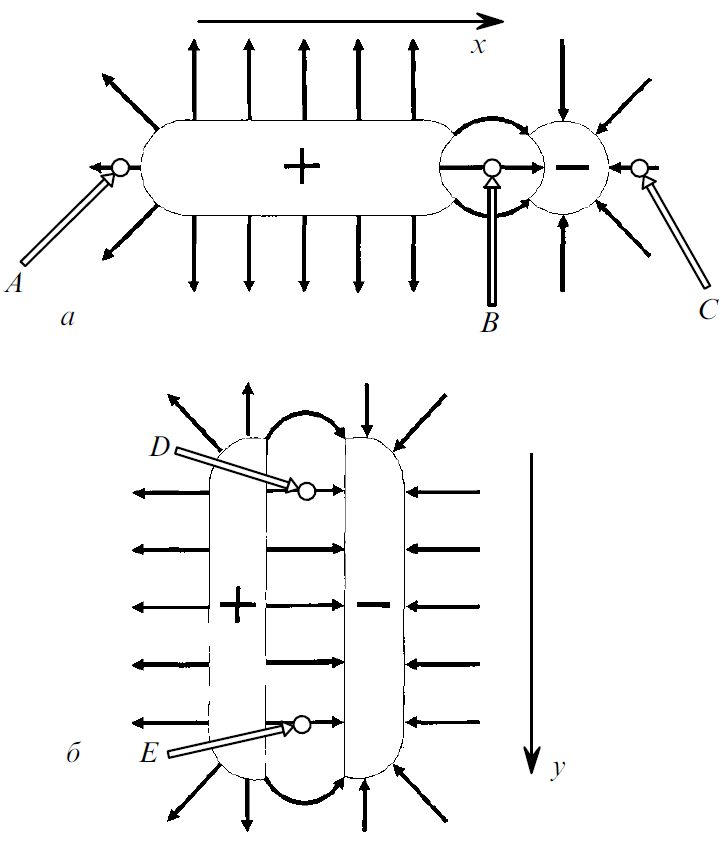
\includegraphics[width=0.5\linewidth]{Dissertation/images/review/expSplit.jpg}
%	\caption{Слева: распределение электрического поля в зарядовой модели при движении пятна света параллельно (а) и перпендикулярно (б) направлению разделения зарядов. Справа: мощность второй гармоники при движении в соответствующих направлениях}
%	\label{fig:expsplit}
%\end{figure}
%
%
%На основании проведённой работы коллектив Диановского волоконного центра предложил и развил зарядовую модель, основанную на анизотропном когерентном фотовольтаическом эффекте \cite{dianov1995photoinduced}.
%
%
%%Как отмечалось в главе про волокно, для достижения волноводного эффекта в световодах посредством увеличения показателя преломления сердцевины волокна необходимо добавлять в плавленый кварц соответствующие примеси. Именно они и являются источником дефектов, приводящих в конечном счёте к фотоиндуцированной генерации второй гармоники.
%%
\subsection{Модель самоорганизации экситонов с переносом заряда}\label{subsec:shg_model}
%\nomenclature{ЭПЗ}{Экситоны с переносом заряда}
%В 2000 году была предложена физическая модель, объединяющая зарядовые и ориентационные особенности предыдущих моделей \cite{antonyuk2001self}. Проводя анализ спектров комбинационного, гиперкомбинационного и люминесцентного спектра оптического волокна, легированного оксидом германия, авторы предложили модель усиления слабого затравочного поля, основанную на самоорганизации возбуждений в среде. Согласно этой модели, примесный электрон, находящийся на Ge-центре поглощает один квант волны второй гармоники (зелёный свет) и переходит либо на другой Ge-центр, либо в силикатную матрицу.  Создаётся \textsf{экситон с переносом заряда (ЭПЗ)}, представляющий собой электрический диполь. Рассматривая электрон-дырочную кинетику в среде, авторы пришли к выводу, что экситоны с переносом заряда представляют собой систему с обратной положительной связью и ориентируются в слабом постоянном электрическом поле так, чтобы его усилить до величины $E\approx10^5~\text{В}/\text{см}$.
%%
%Далее авторы объединяют свою модель с уже существующими, рассматривая усиление слабой волны второй гармоники в периодическом (по длине) электрическом поле, созданным экситонами с переносом заряда. Учёт истощения накачки приводит к первому в мире правильному объяснению временной зависимости эффективности генерации, а также резкому увеличению мощности с последующим спадом при изменении фазовых соотношений между волнами накачки и второй гармоники.
%
%Представим изложенную логику генерации второй гармоники в виде схемы:
%\begin{figure}[h]
%	\centering
%	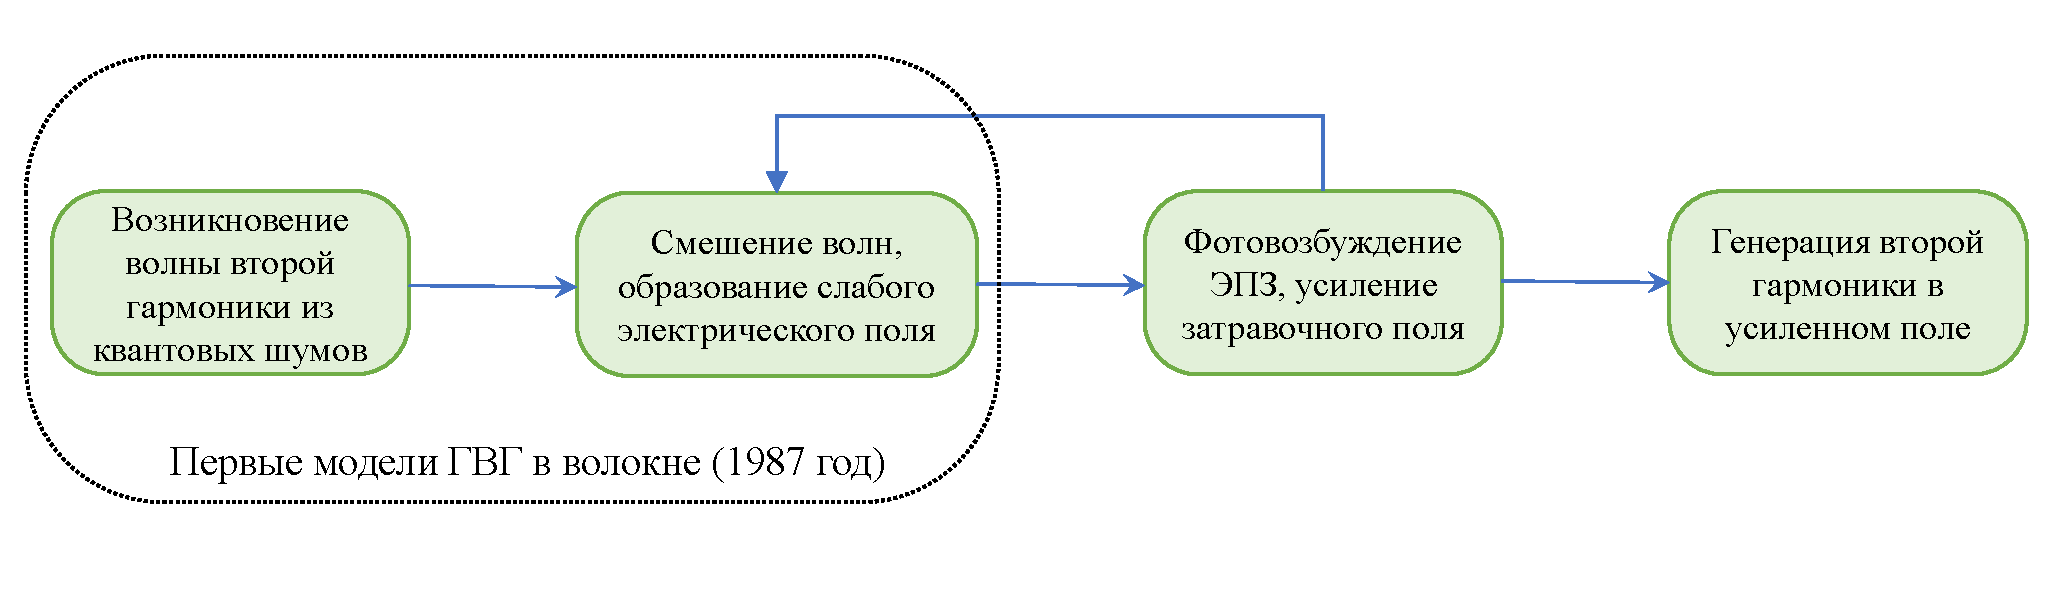
\includegraphics[width=0.99\linewidth]{Dissertation/images/review/scheme_epz}
%	\caption{Упрощённая схема физических процессов при генерации второй гармоник в волокне согласно \cite{antonyuk2001self}}
%	\label{fig:schemeepz}
%\end{figure}
%Как следует из схемы, изображённой на рис. \ref{fig:schemeepz}, в предложенной автором модели находят отражение первые теоретические объяснения эффекта, изложенные сразу после его экспериментального наблюдения.
%
%\subsection{Где там решетка находится}
%\subsubsection{Бартдорф}
%Работа \cite{batdorf1989study}: зависимость мощности ГВГ от длины волокна в стационарном случае. Результаты:
%\begin{itemize}
%	\item Начальная скорость роста не зависит от мощности seed зеленого
%	\item Длина, на которой начинается ГВГ (расстояние от начала волокна до точки, где 10\% от уровня насыщения) (cut-back) зависит от мощности seed зеленого: чем зеленого на входе больше, тем меньше это расстояние. Эмпирическая формула: $L_0 = 7.63 - 1.18 \ln(P_{\text{green}})$. Из интересного - это дает оценку на мощность зелени при self-seeding в пВт.
%	\item Степенная зависимость мощности от длины также будет разной при разных мощах зеленого на входе: чем зеленого на входе меньше, тем эта степень выше. Степень меняется от 2 до 13.
%	\item Насыщение по длине возникает не из-за ФСМ или дисперсии
%\end{itemize}
%Чел лох так как считает что форма зависимости Psh(L) не меняется со временем, а меняется только масштаб (У антонюка так???) Или не лох?
%
%\subsubsection{Лацерда паяльник}
%Работы \cite{lacerda1993self, lacerda1994grating}. 
%В статье 1993 более подробно. Пацаны возникали паяльником по волокну и по результатам возюкания восстанавливали профиль хи2. Из важного: огромная часть экспериментов без сидинга. Результаты шокируют: решетка сначала у входа, затем едет к выходу, в насыщении слабенько едет снова ко входу. Наличие ширины связывается с шириной спектра лазера. Насыщение связывается с неким самостиранием и про фазу самой решетки молчок. Еще они обнаружили что если "читать" не той же мощой что и светили то можно получить какие угодно результаты и на основе этого сделали вывод что ФСМ дает определенный (пи пополам радиан на длине решетки) фазовый СДВГ
%Если сравнить картинки с наличием сидинга и без, то качественное согласие с бартдорформ есть: без сидинга решетка дальше, чем с ним.
%Эволюция положения пика решётки
%В самоинициируемом (self-seeded) режиме пик решётки движется от входного конца к выходному в процессе подготовки, проходя до 20–25 см.
%
%При насыщении эффективности преобразования пик начинает двигаться обратно ко входу, смещаясь на ~2–3 см.
%
%В режиме с внешним затравкой (externally seeded) пик решётки остаётся у входного конца волокна, так как уровень второй гармоники постоянен по длине.
%
%При прерывании внешней затравки пик начинает смещаться внутрь волокна, но не так далеко, как в самоинициируемом случае.
%
%Различие в эволюции. Бартдорф утверждает что профиль во время записи не меняется, а паяльник - что меняется.

\clearpage